        \begin{ledgroupsized}[r]{120mm}
                \footnotesize 
                \pstart                
                \noindent\textbf{\"{U}berlieferung:}   
                \pend
                \end{ledgroupsized}
                            \begin{ledgroupsized}[r]{114mm}
                            \footnotesize 
                            \pstart \parindent -6mm
                            \makebox[6mm][l]{\textit{L}}\selectlanguage{ngerman}Konzept: LH XXXVII 3 Bl. 107\textendash112. 3 Bog. 2\textsuperscript{o}. 12 S. zweispaltig. Linke Spalten fortlaufender Text, rechte Spalten Erg\"{a}nzungen und Textkorrekturen. Auf Bl. 107~r\textsuperscript{o} eine Zeichnung obere H\"{a}lfte rechts. Auf Bl. 107 v\textsuperscript{o} eine Zeichnung unten rechts. Auf Bl. 108 v\textsuperscript{o} obere H\"{a}lfte rechts zwei Zeichnungen, davon eine gestrichen. Auf Bl. 109 r\textsuperscript{o} drei Zeichnungen rechts untereinander, die beiden oberen gestrichen. Auf Bl. 109 v\textsuperscript{o} mittig rechts vier Zeichnungen, davon drei gestrichen. Auf Bl. 110 v\textsuperscript{o} obere H\"{a}lfte rechts zwei Zeichnungen nebeneinander. Die linke gestrichene Zeichnung wird nicht berücksichtigt, da es sich um eine erste Skizze der rechten Zeichnung handelt. Auf Bl. 111 r\textsuperscript{o} untere H\"{a}lfte rechts ebenfalls zwei Zeichnungen nebeneinander, die linke gestrichen. Auch hier wird die gestrichene Zeichnung aufgrund fehlender Signifikanz vernachlässigt. Auf Bl. 112 v\textsuperscript{o} zwei Zeichnungen mittig rechts nebeneinander. Auf Bl. 110 r\textsuperscript{o} obere H\"{a}lfte rechts die Multiplikation zweier Faktoren als Nebenrechnung. 
 \\Cc 2, Nr. 486 B \pend
                            \end{ledgroupsized}
                %\normalsize
                \vspace*{5mm}
                \begin{ledgroup}
                \footnotesize 
                \pstart
            \noindent\footnotesize{\textbf{Datierungsgr\"{u}nde}: Auch f\"{u}r dieses St\"{u}ck ist der Zeitrahmen durch die Publikation des Huygens'schen Briefes im \cite{00062}\textit{Journal des S\c{c}avans} vom 25. Juli 1672 bestimmt, der gleich am Beginn des Textes erw\"{a}hnt wird. Wie Leibniz im Titel ausf\"{u}hrt, geht es ihm darum, neue Experimente vorzuschlagen, die es m\"{o}glich machen sollen, die Kontroversen hinsichtlich des Luftdrucks zu definieren. Es handelt sich also um \"{U}berlegungen, die bereits eine gewisse Vertrautheit mit dem Gegenstand voraussetzen, so dass wir von einer Entstehungszeit des Textes im Herbst 1672 ausgehen.}
                \pend
                \end{ledgroup}
            
                \vspace*{8mm}
                \pstart 
                \normalsize\selectlanguage{latin}
            \begin{center}[107 r\textsuperscript{o}] Propositio Experimentorum Novorum,\\quibus sumtis omnes controversiae\\circa Aeris pressionem\protect\index{Sachverzeichnis}{pressio!aeris}\\videntur definiri \edtext{posse.\edlabel{poss107r1}}
            {\lemma{posse.}\xxref{poss107r1}{poss107r2}\Afootnote{ \textit{ (1) }\ Cum nuper Illustris Hugenius\protect\index{Namensregister}{\textso{Huygens} (Hugenius, Vgenius, Hugens, Huguens), Christiaan 1629\textendash 1695|textit} in novissimo Diario Eruditorum Experimentis rem literariam auxerit \textit{ (2) }\ Experimenta Pneumatica quibus  \textit{(a)}\ Illustris Hugenius\protect\index{Namensregister}{\textso{Huygens} (Hugenius, Vgenius, Hugens, Huguens), Christiaan 1629\textendash 1695|textit} publicatis in novissimo Diario Eruditorum \textit{(b)}\ in \lbrack ...$\rbrack$ auxit \textit{ L}}}
            \end{center}
            \pend 
            \clearpage
            \pstart \edtext{Experimenta Pneumatica quibus in novissimo Diario Eruditorum}{\lemma{Eruditorum}\Bfootnote{\textsc{Chr. Huygens, }\cite{ref}\cite{00062}\textit{Extrait d'une lettre}, \textit{JS} (1672), S.~133\textendash140 (\textit{HO} VII, S.~201\textendash206).}}
            publicatis Illustris Hugenius rem literariam auxit \edlabel{poss107r2} 
        %     \edtext{publicatis Illustris Hugenius rem literariam auxit}{\lemma{posse.}\xxref{poss107r1}{poss107r2}\Afootnote{ \textit{ (1) }\ Cum nuper Illustris Hugenius\protect\index{Namensregister}{\textso{Huygens} (Hugenius, Vgenius, Hugens, Huguens), Christiaan 1629\textendash 1695|textit} in novissimo Diario Eruditorum Experimentis rem literariam auxerit \textit{ (2) }\ Experimenta Pneumatica quibus  \textit{(a)}\ Illustris Hugenius\protect\index{Namensregister}{\textso{Huygens} (Hugenius, Vgenius, Hugens, Huguens), Christiaan 1629\textendash 1695|textit} publicatis in novissimo Diario Eruditorum \textit{(b)}\ in \lbrack ...$\rbrack$ auxit \textit{ L}}},
             admonuere me \edtext{Experientiarum}{\lemma{me}\Afootnote{ \textit{ (1) }\ eorum \textit{ (2) }\ Experientiarum \textit{ L}}} quas in eam rem sum dudum meditatus, et quarum successus omnes ejus argumenti controversias firma demonstratione dirimere posse videtur. Haec publice proponere operae pretium visum est, ut aliis alia pro cujusque commoditate sumentibus, quamprimum \edtext{residuis}{\lemma{}\Afootnote{residuis \textit{ erg.} \textit{ L}}} dubitationibus \edtext{\edlabel{libe107r1}liberemur.} 
             {\lemma{liberemur.}\xxref{libe107r1}{libe107r2}\Afootnote{ \textit{ (1) }\ \textso{Experim. 1.} \textit{ (2) }\   \textbar\ Nec vereor ne quis parum probet Experimenta nondum sumta proponi; \textit{ gestr.}\ \textbar\  Est enim in Experimentis potissimum, ipsa inventio  \textit{(a)}\ ad certum finem directa \textit{(b)}\ non casu, sed certo consilio ac methodo ad naturam e latebris protrahendam directa \textit{(c)}\ si  \textit{(aa)}\ non casu occurrunt, sed \textit{(bb)}\ occurrunt certo consilio ac methodo ad naturam e latebris protrahendam dirigantur.  \textit{(aaa)}\ Et interesset Rei publicae \textit{(bbb)}\ Quare optandum esset directiones Experimentorum faciendorum etiam ab illis proponi qui exequendi \textit{ (3) }\  \textso{Experim. 1.} \textit{ L}}} 
             \pend  
% Zeitz auskommentiert            %\newpage
%          %   \rule[0cm]{0cm}{3cm}  
%             \begin{center}        %           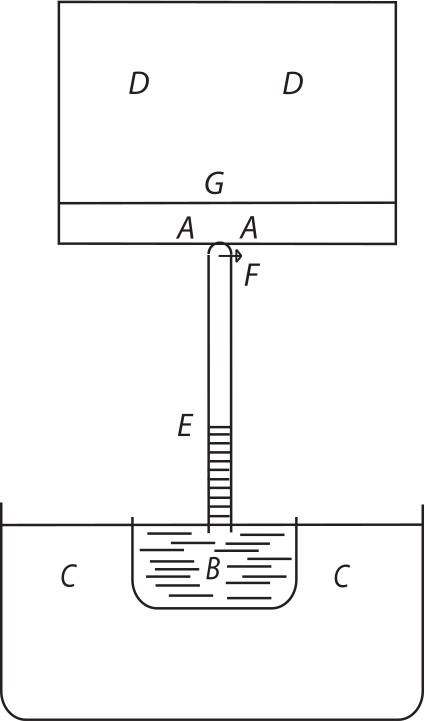
\includegraphics[width=0.37\textwidth]{images/37_3_107r}\\\textit{[Fig. 1]}
%                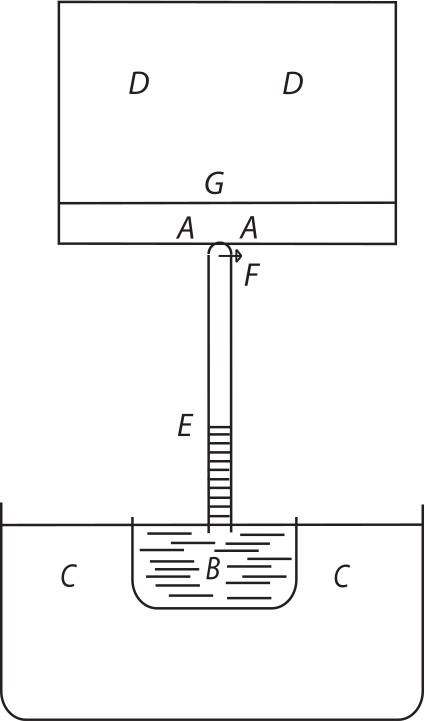
\includegraphics[width=0.33\textwidth]{images/37_3_107r}\\\textit{[Fig. 1]}
%                        %\caption{Bildbeschreibung}
%                        \end{center}
%                        %@ @ @ Dies ist eine Abstandszeile - fuer den Fall, dass mehrere figures hintereinander kommen, ohne dass dazwischen laengerer Text steht. Dies kann zu einer Fahlermeldung fuehren. @ @ @ \\
%                        \newpage
                \pstart          \textso{Experim. I.}
                Esto \edtext{\edlabel{libe107r2}in aere libero}{\lemma{}\Afootnote{in aere libero \textit{ erg.} \textit{ L}}} Tubus Torricellianus\protect\index{Sachverzeichnis}{Tubus!Torricellianus} Mercurio\protect\index{Sachverzeichnis}{mercurius} plenus \textit{AB} vas subjectum in quo stagnat alius Mercurius\protect\index{Sachverzeichnis}{mercurius} \textit{C}. 
 \edtext{Altitudo Mercurii dalabentis \textit{BE}.}{\lemma{\textit{C}.}\Afootnote{ \textit{ (1) }\ Mercurius\protect\index{Sachverzeichnis}{mercurius|textit} ex \textit{AB} delabatur in vas subjectum \textit{C} ita ut non nisi altitudo ordinaria \textit{EB} residua sit summitas \textit{ (2) }\ Altitudo Mercurii dalabentis \textit{BE}. \textit{ L}}} Vas \edtext{bene}{\lemma{}\Afootnote{bene \textit{ erg.} \textit{ L}}} clausum aere ordinario plenum \textit{D} in quod intret \edtext{\textit{A}}{\lemma{}\Afootnote{\textit{A} \textit{ erg.} \textit{ L}}} extremitas Tubi \textit{AB} ita tamen ut Epistomium\protect\index{Sachverzeichnis}{epistomium} \textit{F} clausum communicationem neget inter partem Tubi \textit{FB} et residuam partem \textit{AF} apertam in \textit{A} versus vas \textit{D} et clausam per Epistomium\protect\index{Sachverzeichnis}{epistomium} in \textit{F} versus Tubum \textit{FB}. \edtext{Tubi}{\lemma{\textit{FB}.}\Afootnote{ \textit{ (1) }\ Vas \textit{ (2) }\ Tubus \textit{ (3) }\ Tubi \textit{ L}}} pars \textit{FB} sit Mercurio\protect\index{Sachverzeichnis}{mercurius} plena, clausa in \textit{F} et aperta in \textit{B}. Et Tubo erecto Mercurius\protect\index{Sachverzeichnis}{mercurius} effluet in vas subjectum demta altitudine \textit{BE} spatioque \textit{FE} ad sensum Vacuo relicto. Quo facto aperiatur Epistomium\protect\index{Sachverzeichnis}{epistomium} \textit{F} \edtext{et statim iterum claudatur}{\lemma{}\Afootnote{et statim iterum claudatur \textit{ erg.} \textit{ L}}} ajo si eo \edtext{facto}{\lemma{eo}\Afootnote{ \textit{ (1) }\ casu \textit{ (2) }\ facto \textit{ L}}} Mercurius\protect\index{Sachverzeichnis}{mercurius} \edtext{ex parte saltem}{\lemma{}\Afootnote{ex parte saltem \textit{ erg.} \textit{ L}}} \textit{BE} delabitur in Vas \textit{C} veram esse Hypothesin Funiculi\protect\index{Sachverzeichnis}{funiculus} seu Aeris dilatati \textso{attractionem,}\protect\index{Sachverzeichnis}{attractio} sin suspensus maneat veram esse Hypothesin quae \edtext{\textso{a pressione} seu}{\lemma{}\Afootnote{\textso{pressione} seu \textit{ erg.} \textit{ L}}} Gravitate Aeris\protect\index{Sachverzeichnis}{gravitas!aeris} suspensionem Mercurii\protect\index{Sachverzeichnis}{mercurius} in Tubo repetit. Nam \edtext{ex sententia non Francisci Lini tantum, sed et aliorum doctissimorum virorum Mercurius in Tubo \textit{AB} non ultra descendere potest}{\lemma{Nam}\Afootnote{ \textit{ (1) }\ cum ex sententia  \textit{(a)}\ Francisci Lini\protect\index{Namensregister}{\textso{Linus,} Franciscus 1595\textendash 1675|textit} et sectatorum  \textit{(b)}\ non Francisci Lini\protect\index{Namensregister}{\textso{Linus,} Franciscus 1595\textendash 1675|textit} tantum, sed et aliorum doctissimorum virorum Mercurius\protect\index{Sachverzeichnis}{mercurius|textit} in Tubo descendeat non ultra descendere possit \textit{ (2) }\ ex [...] potest \textit{ L}}}, quam aerem aliamve materiam \edtext{tenuem in tubo}{\lemma{}\Afootnote{tenuem in tubo \textit{ erg.} \textit{ L}}} residuam dilatare potest, hinc illi ajunt \edtext{a materiae illius}{\lemma{ajunt}\Afootnote{ \textit{ (1) }\ ab aeris \textit{ (2) }\ a materiae illius \textit{ L}}} ultra tendi negantis resistentia suspendi Mercurium\protect\index{Sachverzeichnis}{mercurius};\edtext{}{\lemma{}\Afootnote{Mercurium;  \textbar\ nec \textit{ gestr.}\ \textbar\ ad \textit{ L}}} ad eandem semper altitudinem \textit{BE} quantacunque sit altitudo Tubi \textit{AB} quia si tubus altior ac proinde dilatatio major, etiam pondus\protect\index{Sachverzeichnis}{pondus} tendens, seu Mercurius\protect\index{Sachverzeichnis}{mercurius} elapsus fuit major, tubus enim \edtext{Mercurio plenus fuit}{\lemma{enim}\Afootnote{ \textit{ (1) }\ seu salte \textit{ (2) }\ fuit plenus \textit{ (3) }\ Mercurio plenus fuit \textit{ L}}}. Et haec sententia non est adeo absurda quam quibusdam prima specie videtur. Nescio enim an ullum facile Experimentum hactenus publicatum reperturus sit, quod hunc Funiculum\protect\index{Sachverzeichnis}{funiculus} \edtext{falsitatis}{\lemma{}\Afootnote{falsitatis \textit{ erg.} \textit{ L}}} convincat. 
 [107 v\textsuperscript{o}] Nam quod in altissimi Montis vertice minor est altitudo Mercurii\protect\index{Sachverzeichnis}{mercurius} suspensi, hujus rationem facile reddere possunt cum supponant, aerem \edtext{licet gravem}{\lemma{}\Afootnote{licet gravem \textit{ erg.} \textit{ L}}} quanto est altior tanto magis esse tensum \edtext{pondere totius massae\protect\index{Sachverzeichnis}{massa}}{\lemma{}\Afootnote{pondere totius massae\protect\index{Sachverzeichnis}{massa} \textit{ erg.} \textit{ L}}}. Ut funis in summo alligatus pondere sui ipsius tenditur ac diducitur: modo scilicet \edtext{summam aeris superficiem aut esse nullam, aeremque expandi per totum Mundum, aut esse in summo velut alligatam,}{\lemma{scilicet}\Afootnote{ \textit{ (1) }\ aerem summum in summo velut certo puncto alligatum \textit{ (2) }\ atmosphaerae\protect\index{Sachverzeichnis}{atmosphaera|textit} superficiem \textit{ (3) }\ summam [...] alligatam, \textit{ L}}} ut scilicet profundius descendere tota columna non possit, etsi possint partes inferiores, ad funis instar columnaeque ei capitello suspensae fulcroque carentis, sibi imaginentur. Posito enim aerem \edtext{altiorem magis}{\lemma{aerem}\Afootnote{ \textit{ (1) }\ in summo \textit{ (2) }\ altiorem magis \textit{ L}}} esse tensum et aerem tensum vim pati, seque remittere conari in statum aequabilem, sequetur aerem tensum attrahere conari; ac proinde \edtext{pugnam}{\lemma{proinde}\Afootnote{ \textit{ (1) }\ Mercurium\protect\index{Sachverzeichnis}{mercurius|textit} \textit{ (2) }\  pugnam \textit{ L}}} oriri inter duos aeres tensos \edtext{inclusum in Tubo \textit{AB} et externum liberum}{\lemma{tensos}\Afootnote{ \textit{ (1) }\ intus in Tubo \textit{AB} et extra merum \textit{ (2) }\ inclusum [...] liberum \textit{ L}}}, ac proinde \edtext{interiori eum tanto magis eripi, quanto exterior est magis tensus.}{\lemma{proinde}\Afootnote{ \textit{ (1) }\ ab interiore minus trahi, minusque proinde \textit{ (2) }\ interiori [...] tensus. \textit{ L}}} Unde etiam ratio reddi posset, cur \edtext{Tubo Torricelliano in Recipiente Magdeburgico posito}{\lemma{cur}\Afootnote{ \textit{ (1) }\ in Experimento Magdeburgico\protect\index{Sachverzeichnis}{experimentum!Magdeburgicum|textit} \textit{ (2) }\ Tubo [...] posito \textit{ L}}} liquor\protect\index{Sachverzeichnis}{liquor} plane descendat, quia ab aere ejus summe tenso attrahatur. Et cur vesica in valle, aut aere \edtext{ordinario}{\lemma{aere}\Afootnote{ \textit{ (1) }\ libero \textit{ (2) }\ ordinario \textit{ L}}} flaccida, in monte aut Recipiente\protect\index{Sachverzeichnis}{Recipiens!Magdeburgicum} exhausto infletur; quia vesica non minus rotundetur, si extus ab omni parte aequaliter tendatur, quam si intus ab omni parte aequaliter prematur. \edtext{Nec experimenta ad eos penitus convincendos sufficiunt, quibus ostensum est  in aere compresso Mercurium esse altiorem, quia ex eorum Hypothesi dici potest aer non patitur vim compressionis\protect\index{Sachverzeichnis}{vis!compressionis}, sed tensionis\protect\index{Sachverzeichnis}{tensio}, et aerem in sclopeto\protect\index{Sachverzeichnis}{sclopetum} ventaneo compressum non sua sponte sed circumjacente extrahente, (quippe tantundem tenso, quantum ille pressus est) erumpere. Et ideo in aere compresso Mercurium\protect\index{Sachverzeichnis}{mercurius} esse altius suspensum, quia aer compressus sit in effectu minus tensus quam ordinarius, ac proinde minus attrahat. Unde aer internus tensus ad se trahens plus efficit. Haec illi, quae nondum satis firma demonstratione convicta sunt.}{\lemma{}\Afootnote{Nec experimenta ad eos   \textbar\  \textit{ (1) }\ firma demonstratione \textit{ (2) }\ penitus \textit{ erg.}\ \textbar\  convincendos sufficiunt, quibus ostensum est \textit{ (1) }\ aerem compressum Tubum esse \textit{ (2) }\  in aere compresso Mercurium esse  altiorem, quia ex eorum Hypothesi  \textbar\ dici potest \textit{ erg.}\ \textbar\  aer [...] sunt. \textit{ erg.} \textit{ L}}} At Experimentum quod hic propono controversiam dirimet. Nam \edtext{}{\lemma{}\Afootnote{Nam  \textbar\ si \textit{ gestr.}\ \textbar\ aperto \textit{ L}}}aperto Epistomio\protect\index{Sachverzeichnis}{epistomium} \textit{F} \edtext{totus aer contentus in vase \textit{D} et parte Tubi \textit{FE} fit unum et dividit se uniformiter per totum spatium \textit{DFE}.}{\lemma{\textit{F}}\Afootnote{ \textit{ (1) }\ aer vasis \textit{D} dividit sese   \textbar\ proportionaliter \textit{ erg.}~\textbar\  inter spatium vasis \textit{AD} \textit{ (2) }\ totus [...] \textit{DFE}. \textit{ L}}} Quanto ergo majus est vas \textit{D} tanto minus tensionis\protect\index{Sachverzeichnis}{tensio} necesse est partibus singulis obvenire, ergo aer in \textit{FE} tensionem\protect\index{Sachverzeichnis}{tensio} retinebit pene nullam. Quod si igitur Mercurius\protect\index{Sachverzeichnis}{mercurius} \textit{BE} tensione\protect\index{Sachverzeichnis}{tensio} funiculi\protect\index{Sachverzeichnis}{funiculus} suspensus est, tanto plus ipsius delabetur, quanto minor reddita est tensio\protect\index{Sachverzeichnis}{tensio}, seu quanto vas \textit{D} est majus. Quod si non eveniet, pro certo habendum est non a tensione\protect\index{Sachverzeichnis}{tensio} aeris interni, sed a pressione externi Mercurium\protect\index{Sachverzeichnis}{mercurius} suspensum teneri, sin eveniet, funiculum\protect\index{Sachverzeichnis}{funiculus} et pressionem aeris\protect\index{Sachverzeichnis}{pressio!aeris} concurrere putandum est.
\pend 